\documentclass{beamer}

\mode<presentation> {
  \usetheme{CambridgeUS}
  \setbeamercovered{transparent}
}

\usepackage[english]{babel}
\usepackage[utf8]{inputenc}
\usepackage{times}
\usepackage[T1]{fontenc}
\usepackage{fontawesome}
\usepackage[backend=biber, style=numeric]{biblatex}
\addbibresource{SeminarTalk.bib}

\title[Wildlife Tracking with IoT]{Using Internet of Things (IoT) Networks for Wildlife Tracking}
\author{Collin Beane}
\institute[U of Minn, Morris]
{
  Division of Science and Mathematics \\
  University of Minnesota, Morris \\
  Morris, Minnesota, USA
}
\date{\today}

\begin{document}

\begin{frame}
  \titlepage
\end{frame}

\begin{frame}
  \frametitle{Hypothetical Scenario}
  \begin{figure}[htbp]
    \centering
    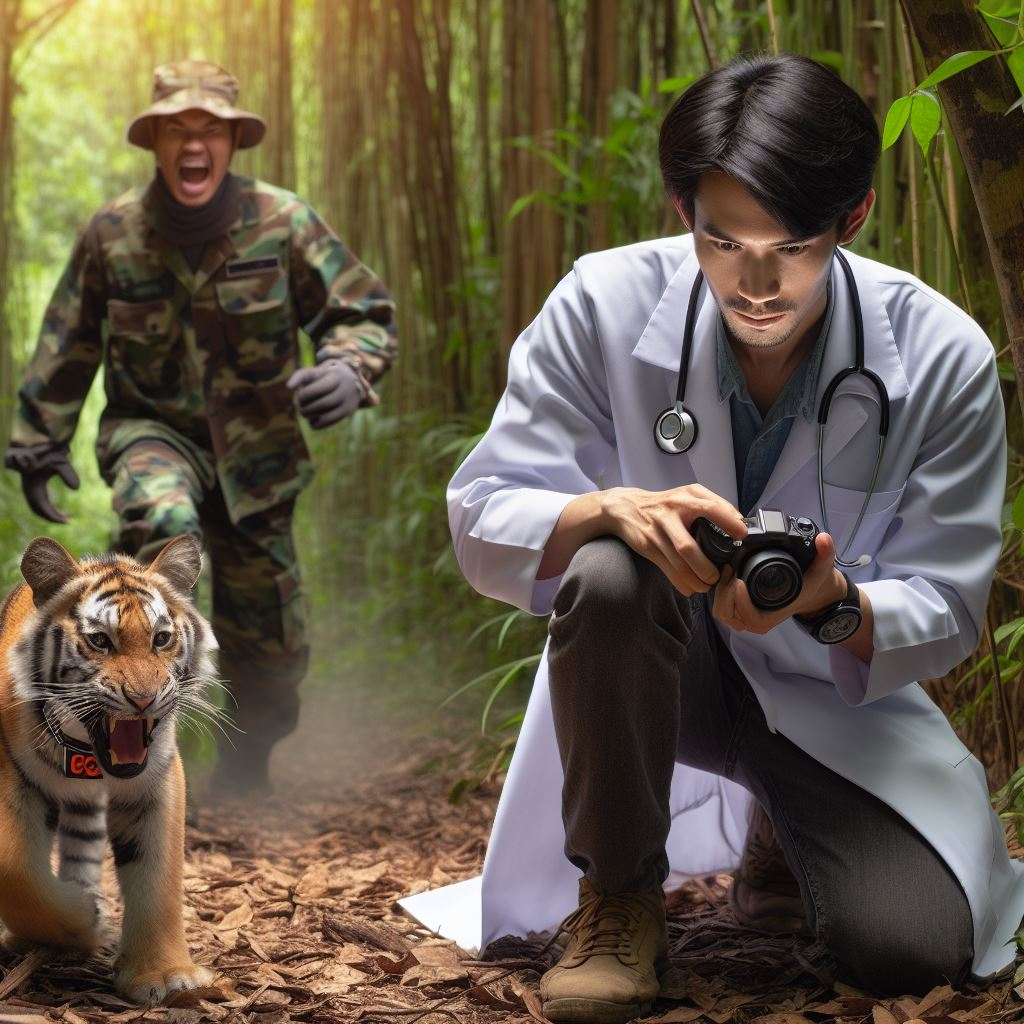
\includegraphics[height=.8\textheight]{Biologging_scenario.jpg}
    \label{fig:Hypothetical_biologging}
  \end{figure}
\end{frame}


\begin{frame}
  \frametitle{Outline}
  \tableofcontents[sectionstyle=show,subsectionstyle=hide]
\end{frame}

% Section and subsections will appear in the presentation overview and table of contents.

\section{Background}

\subsection{What is Biologging?}
\begin{frame}{Background}
  \frametitle{Introduction to Biologging}
        \begin{figure}[htbp]
          \centering
          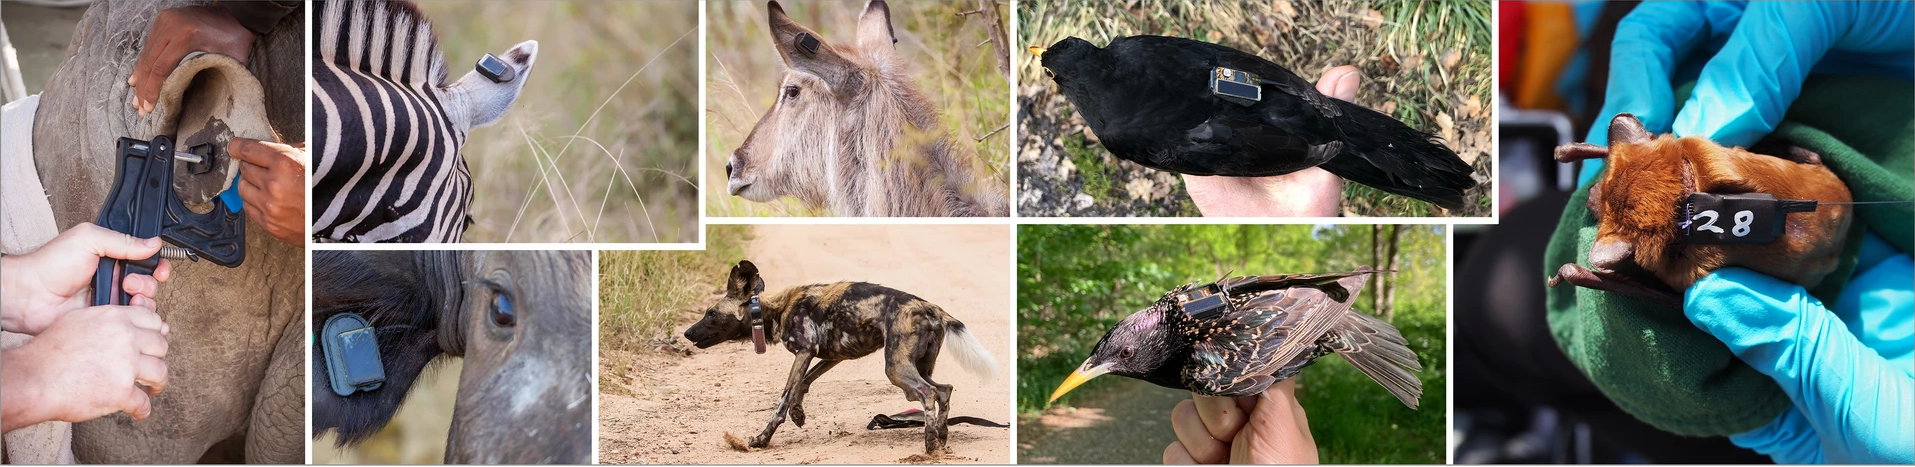
\includegraphics[width=.9\textwidth, height=.25\textheight]{TrakingDevices.png}
          \caption{Animals With SigFox enabled biologging tags \cite{wild2023multi}}
          \label{fig:TaggedAnimals}
        \end{figure}
        \begin{itemize}
          \item Definition: "Investigation of phenomena in or around free-ranging organisms beyond human visibility or experience.\cite{boyd2004bio}"
          \item Method: Tracking wild animals using electronic devices attached to the animal
          \item $\uparrow$ Popularity in early 2000s, practiced since the 60's
          \item Pivotal role in understanding animal behavior and ecology
        \end{itemize}
\end{frame}

\begin{frame}{Background}
  \frametitle{Applications of Biologging}
  \begin{columns}
    \begin{column}{0.5\textwidth}
  \begin{figure}[htbp]
    \centering
    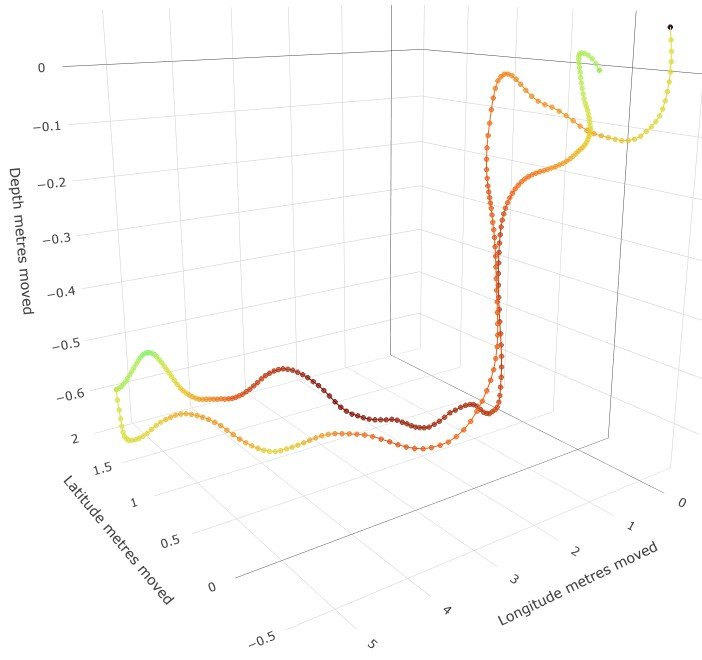
\includegraphics[width=\textwidth]{prairie_dog_map.jpg}
    \caption{3D movement of a prairie dog \cite{Kidangoor_2024}}
    \label{fig:prairie_dog_3D_movement}
  \end{figure}
\end{column}
\begin{column}{0.5\textwidth}
  \begin{itemize}
    \item Track animal movements, behaviors, and migration patterns
    \item Collect data on the animal's environment.
    \item Insights into organisms in hostile or hard-to-reach environments
  \end{itemize}
\end{column}
\end{columns}
\end{frame}

\begin{frame}{Background}
  \frametitle{Impact and Importance}
        \begin{itemize}
          \item Study previously inaccessible aspects of animal life.
          \item Inform conservation efforts and protect endangered species.
          \item Important tool for data collection
          \item Interpretation and application are up to scientists and conservationists.
        \end{itemize}
\end{frame}

\begin{frame}{Background}
  \frametitle{Other Biologging Methods}
  \begin{columns}
    \begin{column}{0.5\textwidth}
        \begin{itemize}
          \item Cellular networks; High Cost
          \begin{itemize}
            \item High Cost/message
          \end{itemize}
          \item Radio Frequency (5-1000m)
          \begin{itemize}
            \item Periodic tracking records
            \item Time stamped data
          \end{itemize}
        \end{itemize}
      \end{column}
      \begin{column}{.5\textwidth}
        \begin{figure}[htbp]
          \centering
          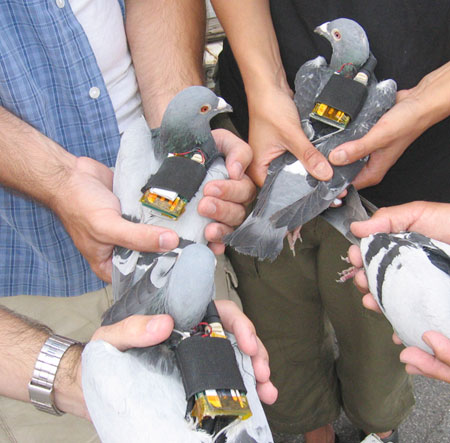
\includegraphics[width=\textwidth]{PigeonCellular.jpg}
          \caption{Pigeons Equipped with cellular trackers \cite{Martin_2006}}
          \label{fig:PigeonCellular}
        \end{figure}
      \end{column}
    \end{columns}
\end{frame}

\subsection{Wireless Networks Basics}

\begin{frame}{Background}
  \frametitle{Data Transmission}
  \begin{columns}
    \begin{column}{0.5\textwidth}
        \begin{figure}[htbp]
          \centering
          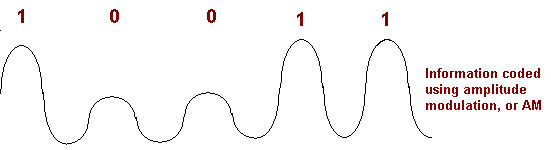
\includegraphics[width=\textwidth]{AMdataTransmission.jpg}
          \caption{How data is represented using amplitude modulation \cite{AMdata}}
          \label{fig:AM_data_transmission}
        \end{figure}
    \end{column}
    \begin{column}{0.5\textwidth}
      \begin{itemize}
        \item Data encoded into 1's and 0's
          \begin{itemize}
            \item Represented by different amplitudes of radio waves
            \item Received and translated by other devices
          \end{itemize}
      \end{itemize}
    \end{column}
  \end{columns}
\end{frame}

\begin{frame}{Background}
  \frametitle{Common Wireless Network Frequencies}
  \begin{columns}
    \begin{column}{0.5\textwidth}
      \begin{itemize}
        \item Home WiFi Frequencies
          \begin{itemize}
            \item 2.4GHz/5GHz/6GHz
          \end{itemize}
        \item LPWAN Frequencies
          \begin{itemize}
            \item $<$1GHz (depends on region)
          \end{itemize}
        \item As frequency increases, range is sacrificed for higher data rates
      \end{itemize}
    \end{column}
    \begin{column}{0.5\textwidth}
      \begin{figure}[htbp]
        \centering
        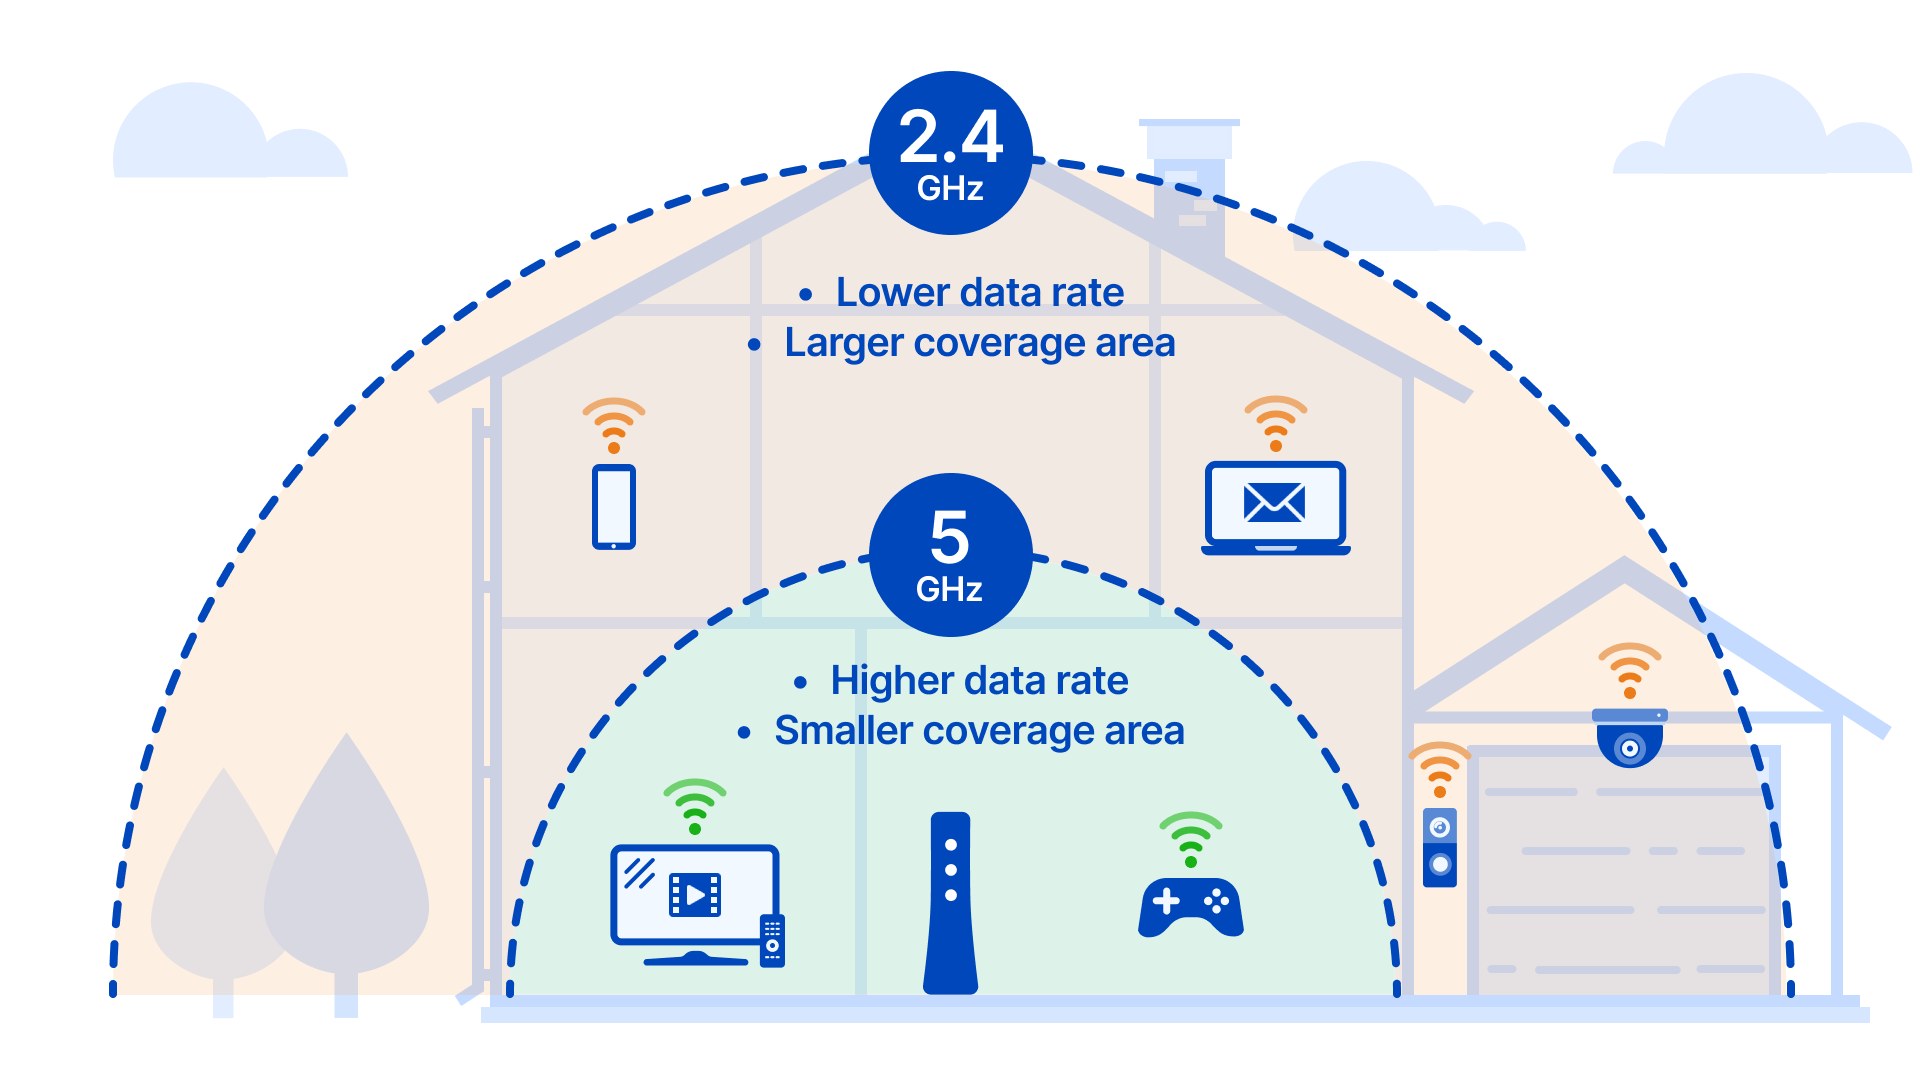
\includegraphics[width=\textwidth]{FreguencyHouse.png}
        \caption{5 GHz will give you more signal strength and faster speed over a shorter range, 
        compared to 2.4 GHz \cite{CenturyLink}}
        \label{fig:FrequencyHouse}
      \end{figure}
  \end{column}
  \end{columns}
\end{frame}

\begin{frame}{Background}
  \frametitle{Concepts of Wireless Frequencies}
  \begin{columns}
    \begin{column}{0.5\textwidth}
        \begin{figure}[htbp]
          \centering
          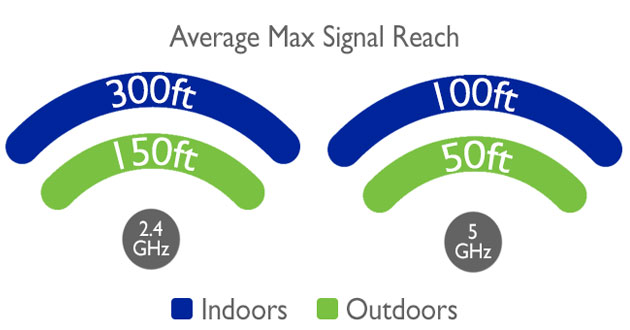
\includegraphics[height=.3\textheight]{WiFi-frequency-reach.jpg}
          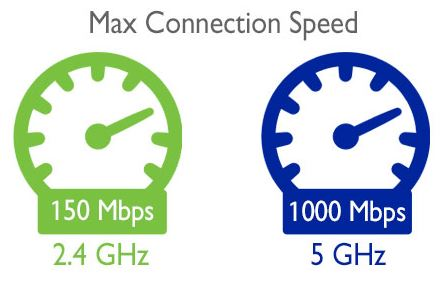
\includegraphics[height=.3\textheight]{WiFi-frequency-speed.jpg}
          \caption{Comparing Range \& Speed of frequencies \cite{WiFiFreqImOn}}
          \label{fig:WiFi-frequency-speed}
        \end{figure}
    \end{column}
    \begin{column}{0.5\textwidth}
          \begin{itemize}
            \item Higher frequency $\Rightarrow$ higher data rates 
              \begin{itemize}
                \item more ones and zeroes received per second
              \end{itemize}
            \item Range is more important than speed in some Applications
            \item Lower frequencies can reach 10's of km vs. 100's of m
          \end{itemize}
    \end{column}
  \end{columns}
\end{frame}

\subsection{What is the Internet of Things?}

\begin{frame}{Background}
  \frametitle{What is the Internet of Things?}
  \begin{itemize}
    \item Empowering physical objects with sensors and software for autonomous interaction
    \item Can either connect via wired or wireless connection
    \item Many applications: Healthcare, agriculture, and of course conservation
  \end{itemize}
\end{frame}

\begin{frame}{Background}
  \frametitle{Layers of an IoT System}
  \begin{columns}
    \begin{column}{0.6\textwidth}
      \begin{itemize}
        \item Application Layer
          \begin{itemize}
            \item Processes and uses data
          \end{itemize}
        \item Network Layer
          \begin{itemize}
            \item Establishes connection to internet and IoT devices
            \item Transmits data to and from the other layers
          \end{itemize}
        \item Perception Layer
          \begin{itemize}
            \item Collects data from the environment or...
            \item Interacts with the physical device
          \end{itemize}
      \end{itemize}
    \end{column}
    \begin{column}{0.4\textwidth}
      \begin{figure}[htbp]
        \centering
        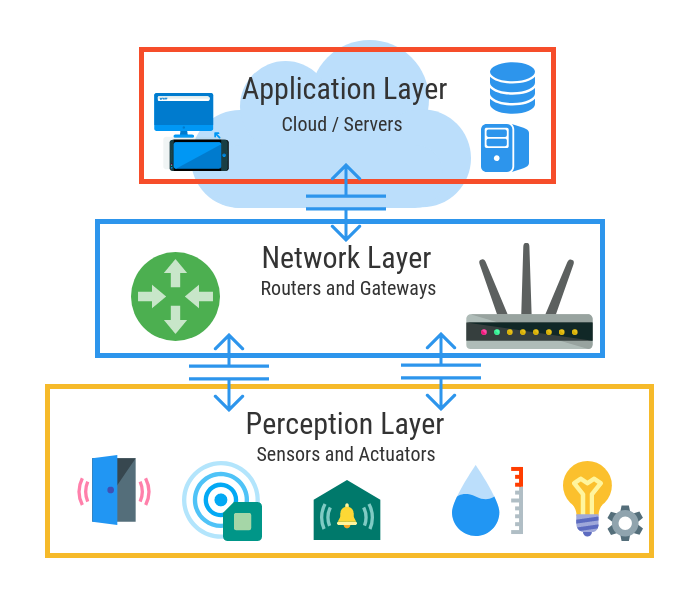
\includegraphics[width=\textwidth]{three-layer-iot-architecture.png}
        \caption{Layer Structure of an IoT System \cite{Calihman_2021}}
        \label{fig:IoT_Layers}
      \end{figure}
  \end{column}
  \end{columns}
\end{frame}



\section{Components of a Modern Biologging System}

\subsection{Sensor Devices}

  \begin{frame}{Components of a Modern Biologging System}
    \frametitle{Sensor Devices}
    \begin{columns}
      \begin{column}{.5\textwidth}
        \begin{itemize}
          \item Required Components
          \begin{itemize}
            \item Antenna
            \item Microcontroller
            \item Battery
            \item Sensor(s)
          \end{itemize}
          \item Optional Components
          \begin{itemize}
            \item Solar panel
            \item Extra storage
          \end{itemize}
        \end{itemize}
      \end{column}
      \begin{column}{0.5\textwidth}
        \begin{figure}[htbp]
          \centering
          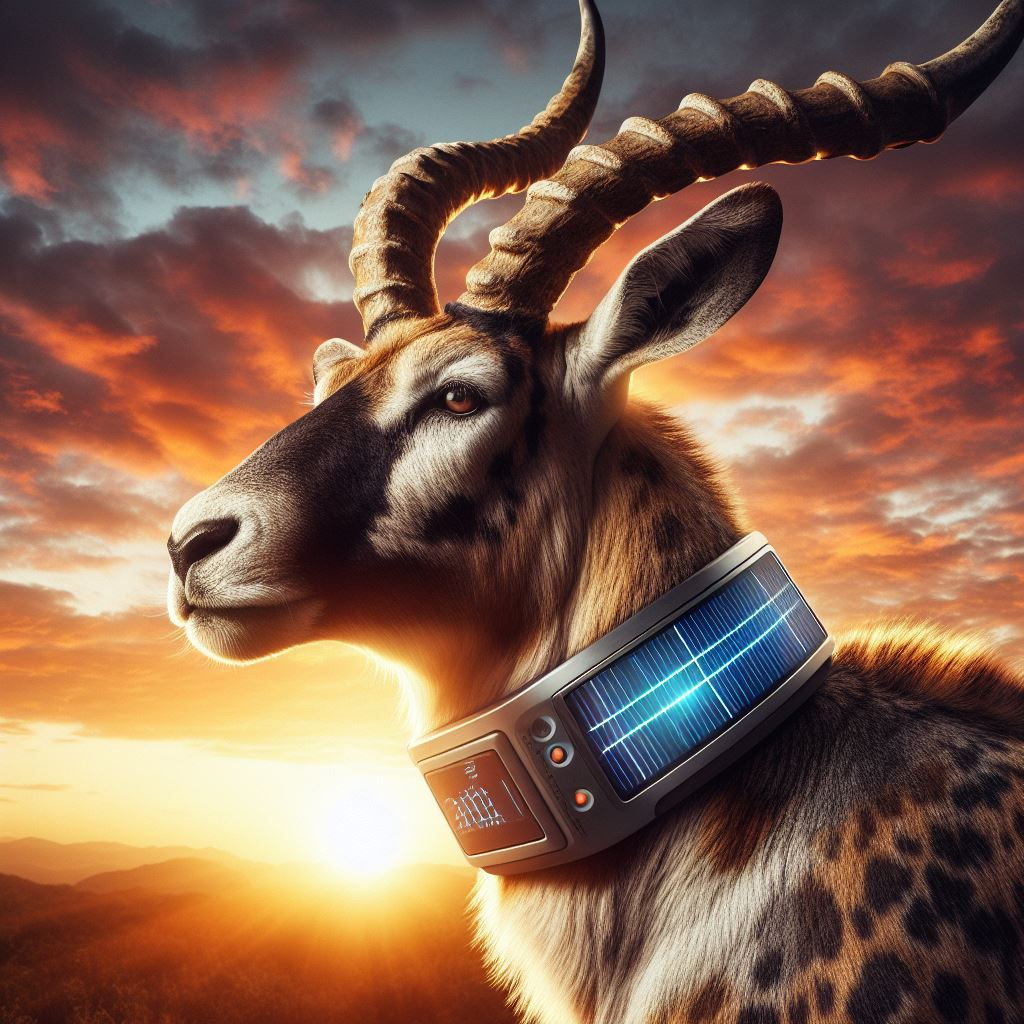
\includegraphics[height=.6\textheight]{Solar_collar.jpg}
          \caption{Animal wearing a solar powered biologging collar, looking majestic [DALL$\cdot$E 3]}
          \label{fig:Solar_collar}
        \end{figure}
    \end{column}
    \end{columns}
  \end{frame}

  \begin{frame}{Components of a Modern Biologging System}
    \frametitle{Sensor Devices}
    \begin{figure}[htbp]
      \centering
      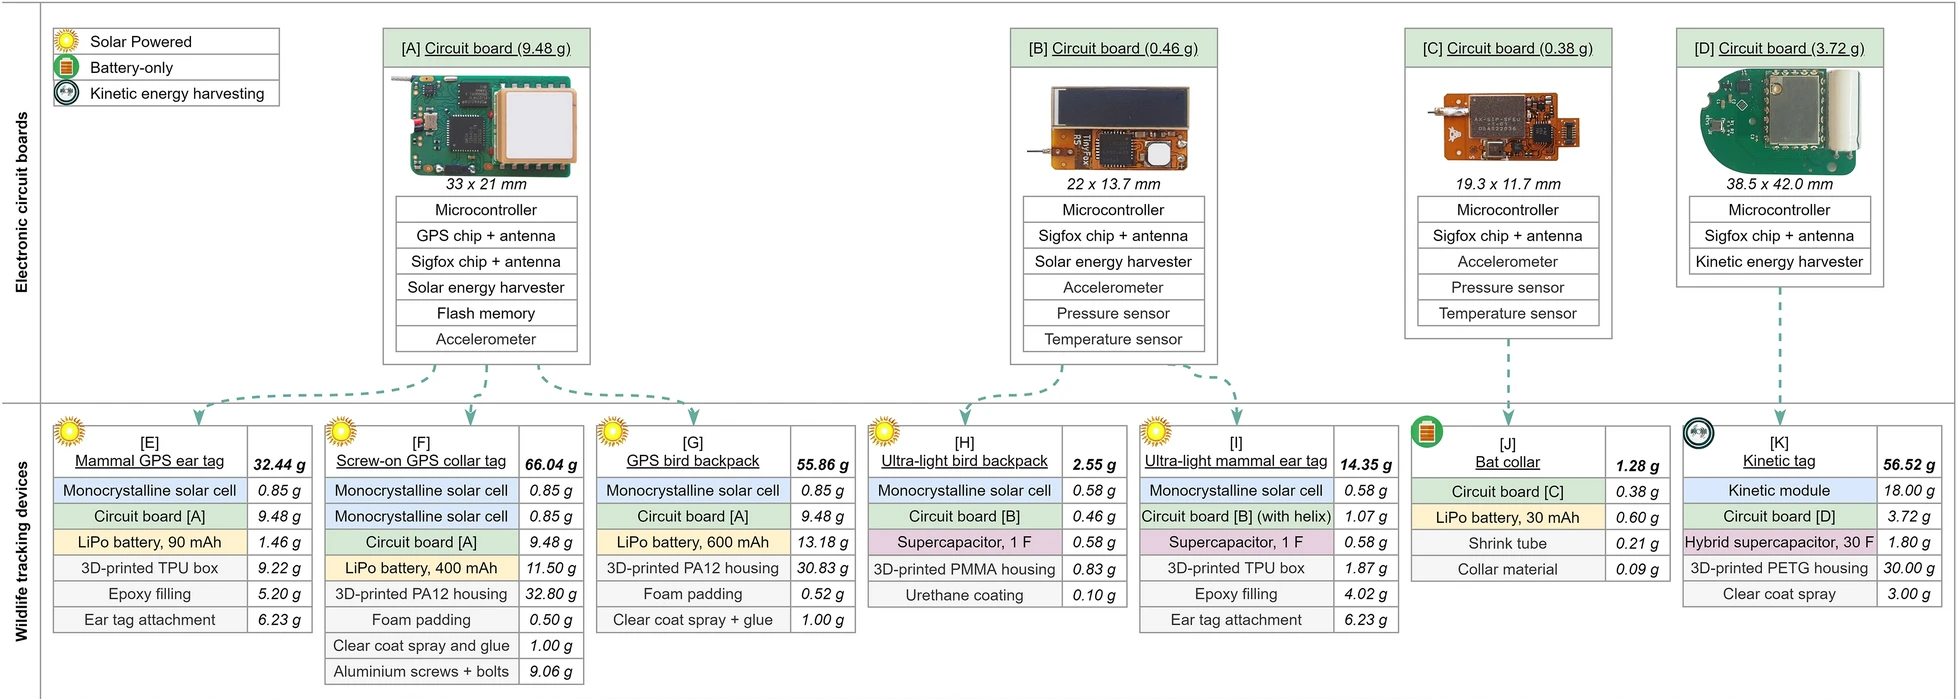
\includegraphics[width=\textwidth]{SigFox_Sensor_device.png}
      \caption{SigFox Biologging Sensor Device \cite{wild2023multi}}
      \label{fig:SigFox_Biologging_device}
    \end{figure}
  \end{frame}

\subsection{Base Stations}

  \begin{frame}{Components of a Modern Biologging System}
    \frametitle{Base Stations}
    \begin{columns}
      \begin{column}{0.4\textwidth}
        \begin{figure}[htbp]
          \centering
          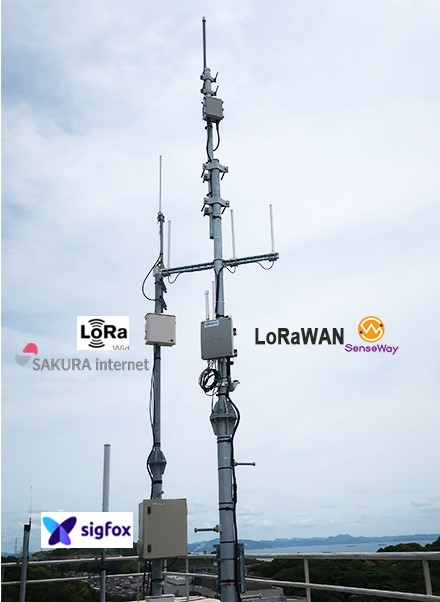
\includegraphics[height=.6\textheight]{BaseStation.jpg}
          \caption{YRP base station \cite{miyajima_2020}}
          \label{fig:LPWAN_Base_Station}
        \end{figure}
      \end{column}
      \begin{column}{0.6\textwidth}
        \begin{itemize}
          \item RF Receiver and transmitter
          \item Connection to internet
          \item Packet forwarding engine
          \item Power source
          \item Local Storage (Optional)
        \end{itemize}
      \end{column}
    \end{columns}
  \end{frame}

\section{Networks for a Biologging System}

\subsection{Networking Outline}
  \begin{frame}{Networking}
    \frametitle{Networking Outline}
    \begin{itemize}
      \item Importance of a Strong Network for Biologging
      \item LPWAN Networks
      \begin{itemize}
        \item SigFox
        \item LoRa
      \end{itemize}
      \item WLAN Networks
      \item Security of LPWAN and WLAN Networks
      \item Which Network is Best for Biologging?
    \end{itemize}
  \end{frame}


\subsection{Importance of a Strong Network}
  \begin{frame}{Networking}
    \frametitle{Importance of a Strong Network for Biologging}
    \begin{columns}
      \begin{column}{0.5\textwidth}
        \begin{itemize}
          \item Data must be transmitted safely and securely
          \item Responsible for sending data to and from sensor device to application layer
        \end{itemize}
      \end{column}
      \begin{column}{0.5\textwidth}
        \begin{figure}[htbp]
          \centering
          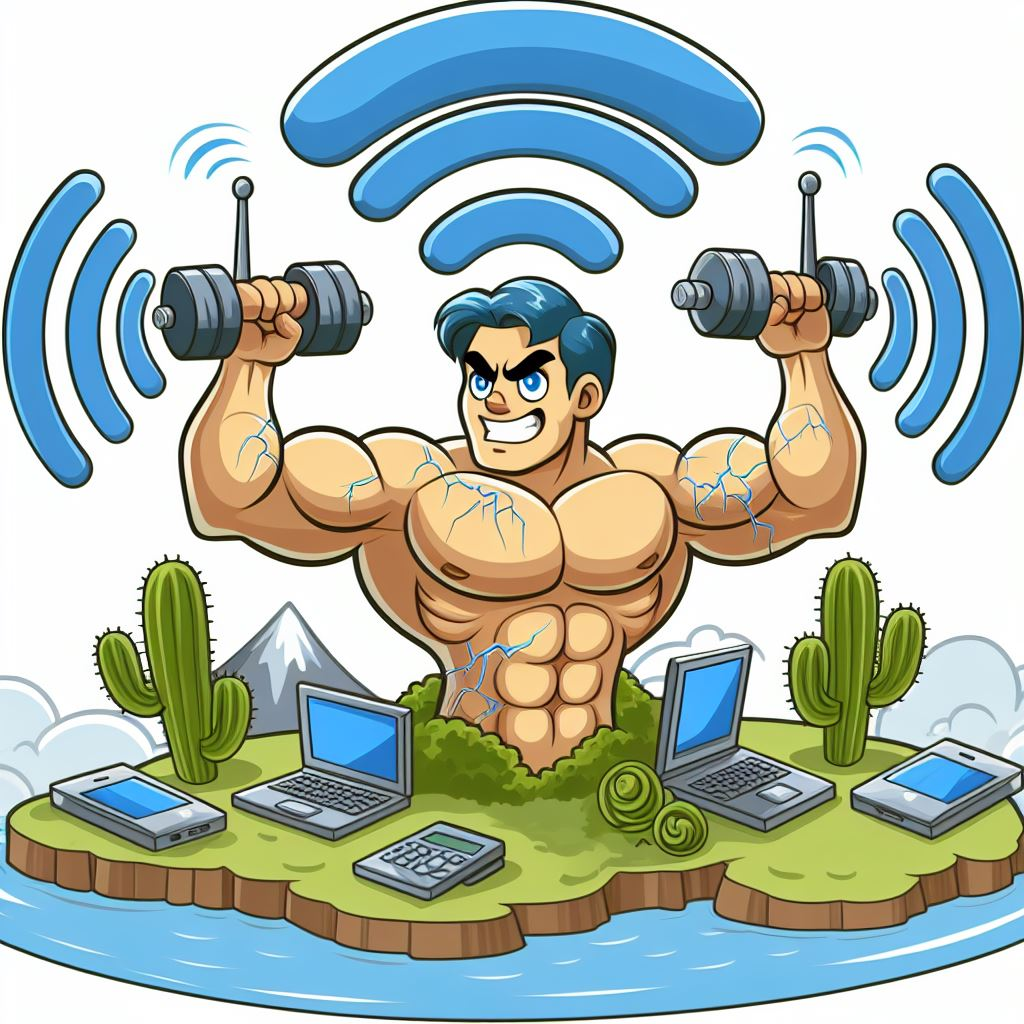
\includegraphics[width=\textwidth]{StrongNetwork.jpg}
          \caption{Cartoon depiction of a strong wireless network [DALL$\cdot$E 3]}
          \label{fig:Strong_wireless_network}
        \end{figure}
      \end{column}
    \end{columns}
  \end{frame}

\subsection{LPWAN Networks}

  \begin{frame}{Networking}
    \frametitle{LPWAN Overview}
    \begin{columns}
      \begin{column}{0.4\textwidth}
        \begin{figure}[htbp]
          \centering
          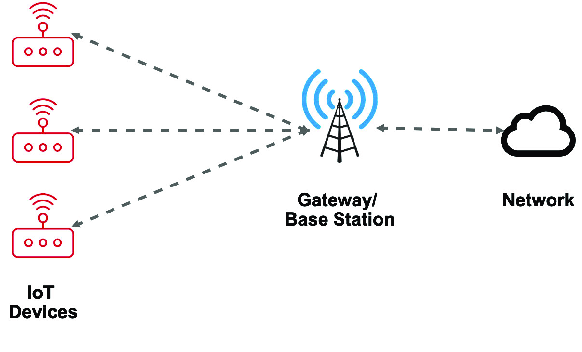
\includegraphics[width=\textwidth]{LPWAN-technologies-network-architecture.png}
          \caption{LPWAN technologies network architecture \cite{LoRaNetworkFernandez}}
          \label{fig:LPWAN_Network_architecture}
        \end{figure}
      \end{column}
      \begin{column}{0.6\textwidth}
        \begin{itemize}
          \item \b{L}ow \b{P}ower \b{W}ide \b{A}rea \b{N}etwork
          \item Utilizes unlicensed Industrial, Scientific and Medical radio bands (ISM)
          \item 433MHz-928MHz Depending on region (U.S. 915MHz)
          \item Very long range (40km+)
          \item Very low power consumption
        \end{itemize}
      \end{column}
    \end{columns}
  \end{frame}

  \begin{frame}{Networking}
    \frametitle{SigFox LPWAN Capabilities}
    \begin{columns}
      \begin{column}{0.5\textwidth}
        \begin{itemize}
          \item 140 messages/day (12bytes each)
          \item 40km+ of range depending on environment
          \item SigFox Atlas technology for estimating location
          \item 6.5yr battery life w/ 2 AAA batteries (more with solar panel)
          \item Up to 100bps
        \end{itemize}
      \end{column}
      \begin{column}{0.5\textwidth}
        \begin{figure}[htbp]
          \centering
          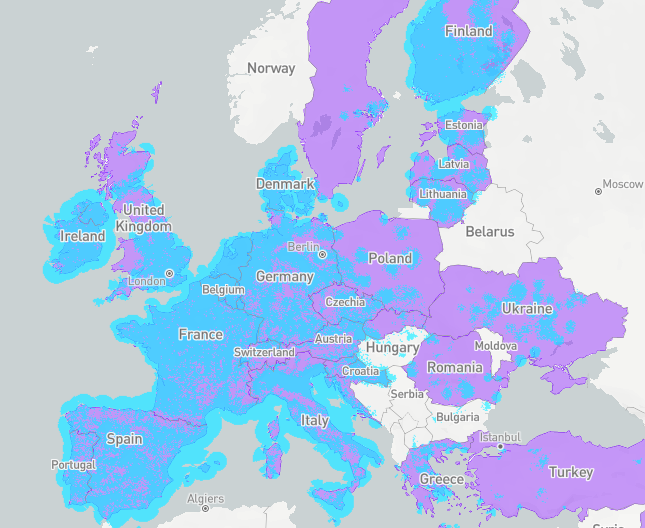
\includegraphics[width=\textwidth]{SigFoxCoverage.png}
          \caption{SigFox Europe Coverage \cite{Sigfox_0G_Technology_2024}}
          \label{fig:SigFox_Coverage}
        \end{figure}
      \end{column}
    \end{columns}
  \end{frame}

  \begin{frame}{Networking}
    \frametitle{SigFox LPWAN Operation}
    \begin{columns}
      \begin{column}{0.5\textwidth}
        \begin{figure}[htbp]
          \centering
          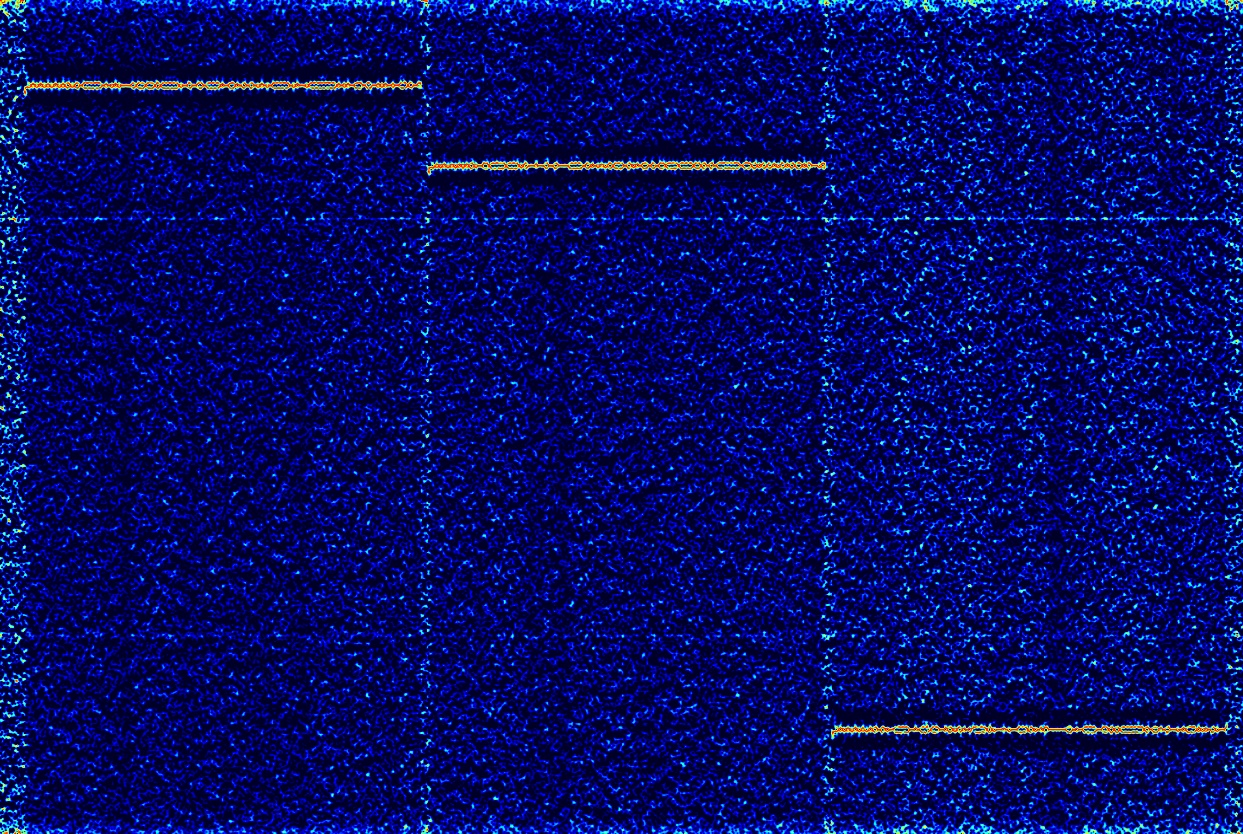
\includegraphics[width=\textwidth]{Sigfox_Spectrum_Analysis.jpg}
          \caption{SigFox frequency hopping modulation \cite{SIGFOXsignalwiki}}
          \label{fig:SigFox_Spectrum}
        \end{figure}
      \end{column}
      \begin{column}{0.5\textwidth}
        \begin{itemize}
          \item Transmission modulation
          \begin{itemize}
            \item transmits message 3 times
            \item pseudo randomly hops to new frequency
          \end{itemize}
          \item Proprietary base stations and framework
          \item Subscription based connection to network
        \end{itemize}
      \end{column}
    \end{columns}
  \end{frame}

  \begin{frame}{Networking}
    \frametitle{LoRa LPWAN Capabilities}
    \begin{columns}
      \begin{column}{0.5\textwidth}
        \begin{itemize}
          \item Unlimited messages/day
          \item Easier to develop and implement
          \item 20km+ of range depending on environment
          \item Up to 50kbps
        \end{itemize}
      \end{column}
      \begin{column}{0.5\textwidth}
        \begin{figure}[htbp]
          \centering
          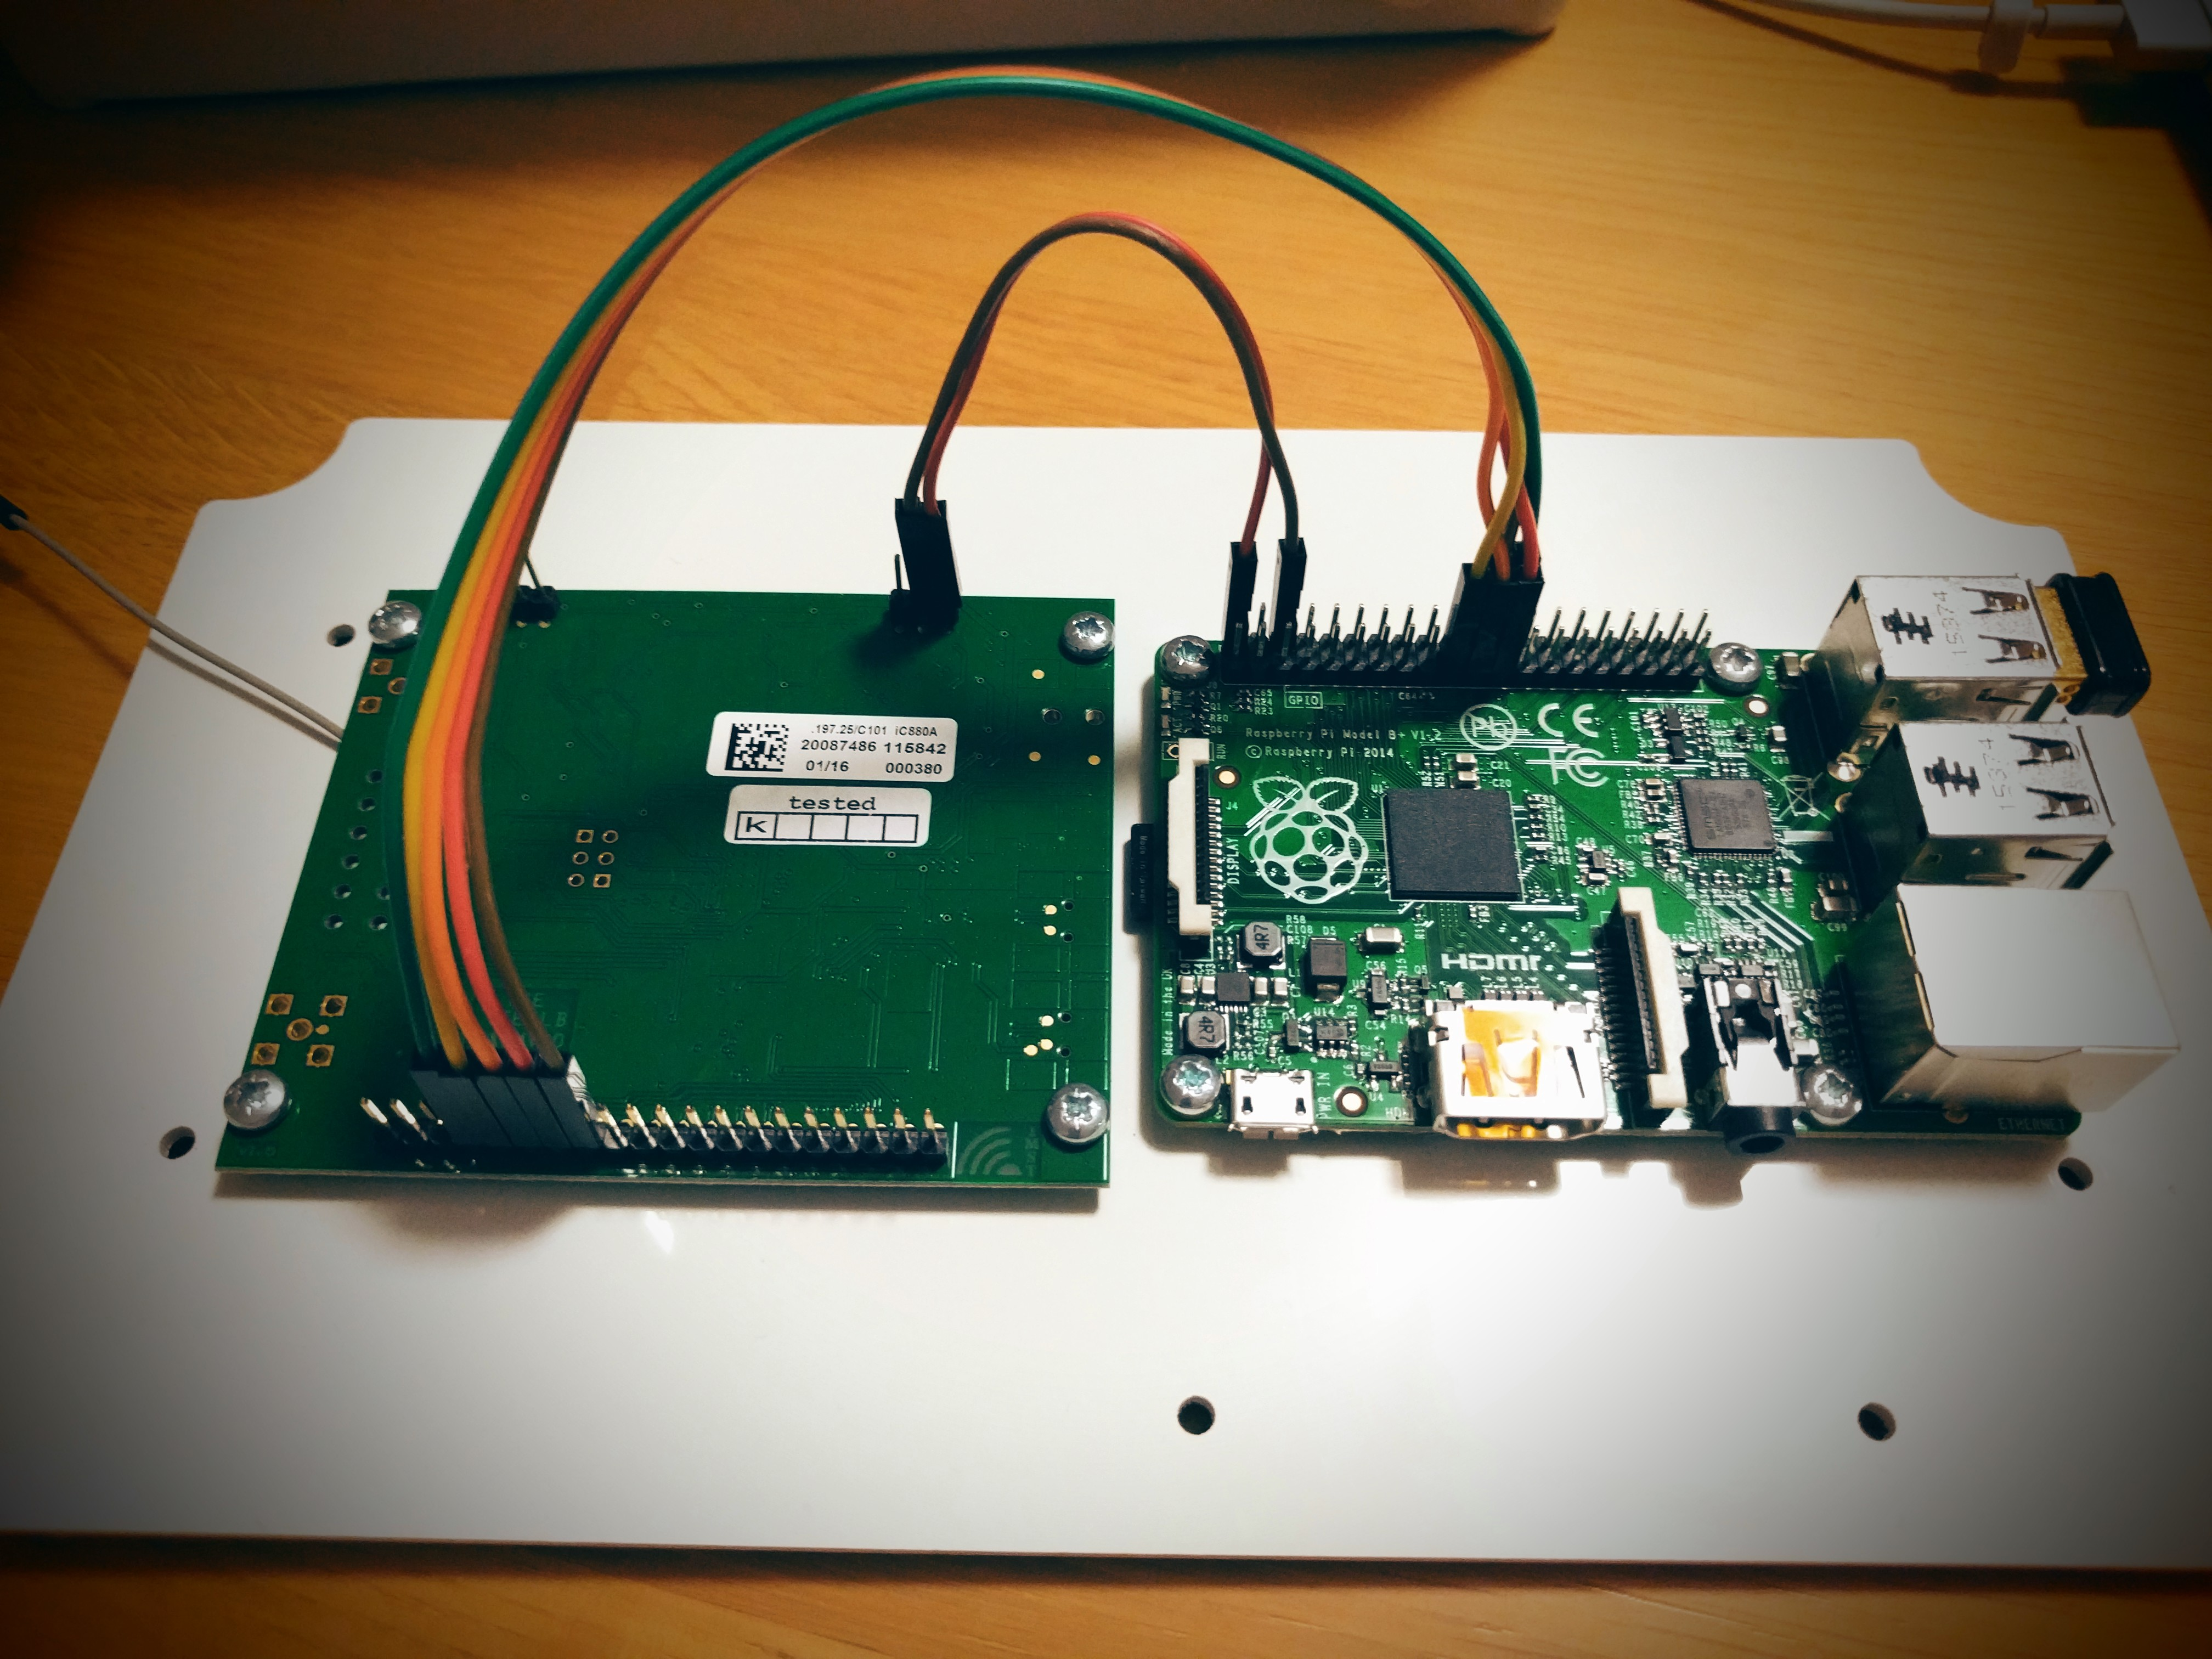
\includegraphics[width=\textwidth]{DIYloraGateway.jpg}
          \caption{DIY LoRa gateway w/ Raspberry Pi \cite{DIYLoRa}}
          \label{fig:DIY_LoRa_Gateway}
        \end{figure}
      \end{column}
    \end{columns}
  \end{frame}

  \begin{frame}{Networking}
    \frametitle{LoRa LPWAN Operation}
    \begin{columns}
      \begin{column}{0.5\textwidth}
        \begin{figure}[htbp]
          \centering
          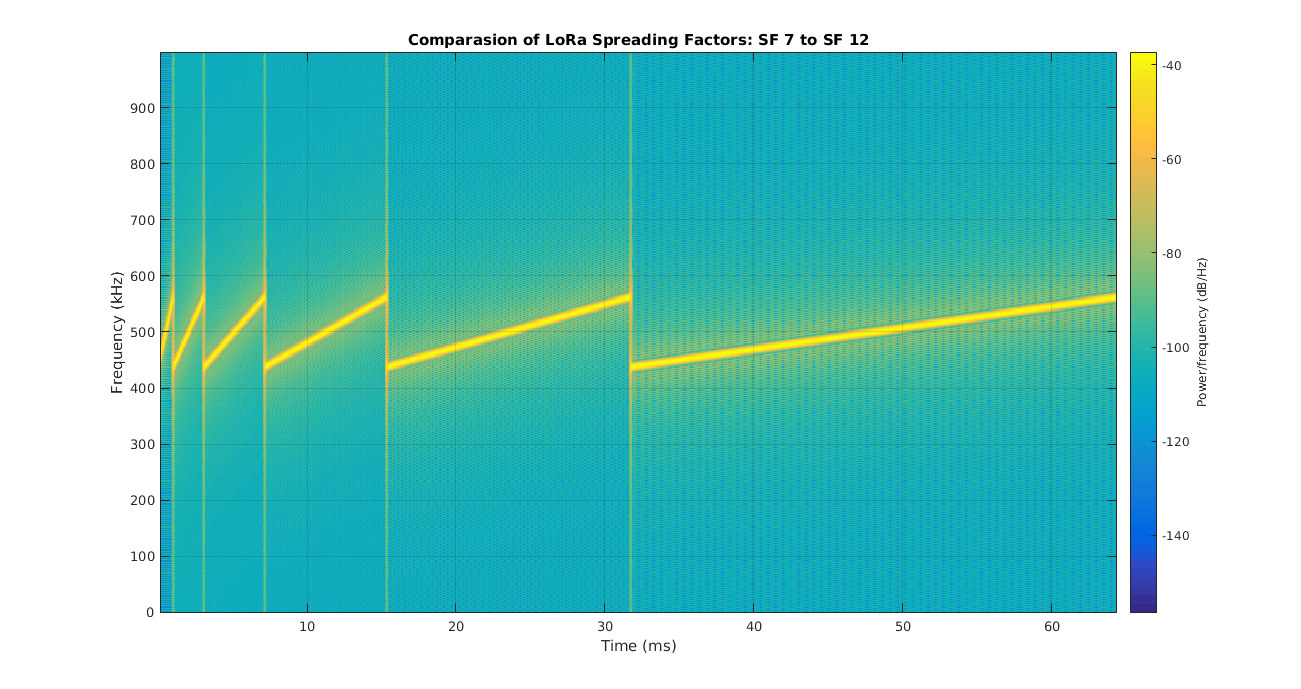
\includegraphics[width=\textwidth]{Chirp.png}
          \caption{CHIRP Spread Spectrum modulation SF7-SF12 \cite{ghoslya2017lora}}
          \label{fig:CHIRP_Spread_Spectrum}
        \end{figure}
      \end{column}
      \begin{column}{0.5\textwidth}
        \begin{itemize}
          \item CHIRP (Compressed High Intensity Radar Pulse) Spread Spectrum
          \begin{itemize}
            \item gradually raises/lowers frequencies
            \item $\uparrow$ SF $\rightarrow$ $\downarrow$ modulation rates
          \end{itemize}
          \item Standards based system
          \item Private or public networks
        \end{itemize}
      \end{column}
    \end{columns}
  \end{frame}

  \begin{frame}{Networking}
    \frametitle{WLAN Capabilities}
    \begin{columns}
      \begin{column}{0.5\textwidth}
        \begin{itemize}
          \item 200m+ of range depending on environment
          \item Unlimited messages/day
          \item 24/7 data transmission
          \item 1840kbps+ (depending on implementation)
          \item Can use any 2.4GHz network
        \end{itemize}
      \end{column}
      \begin{column}{0.5\textwidth}
        \begin{figure}[htbp]
          \centering
          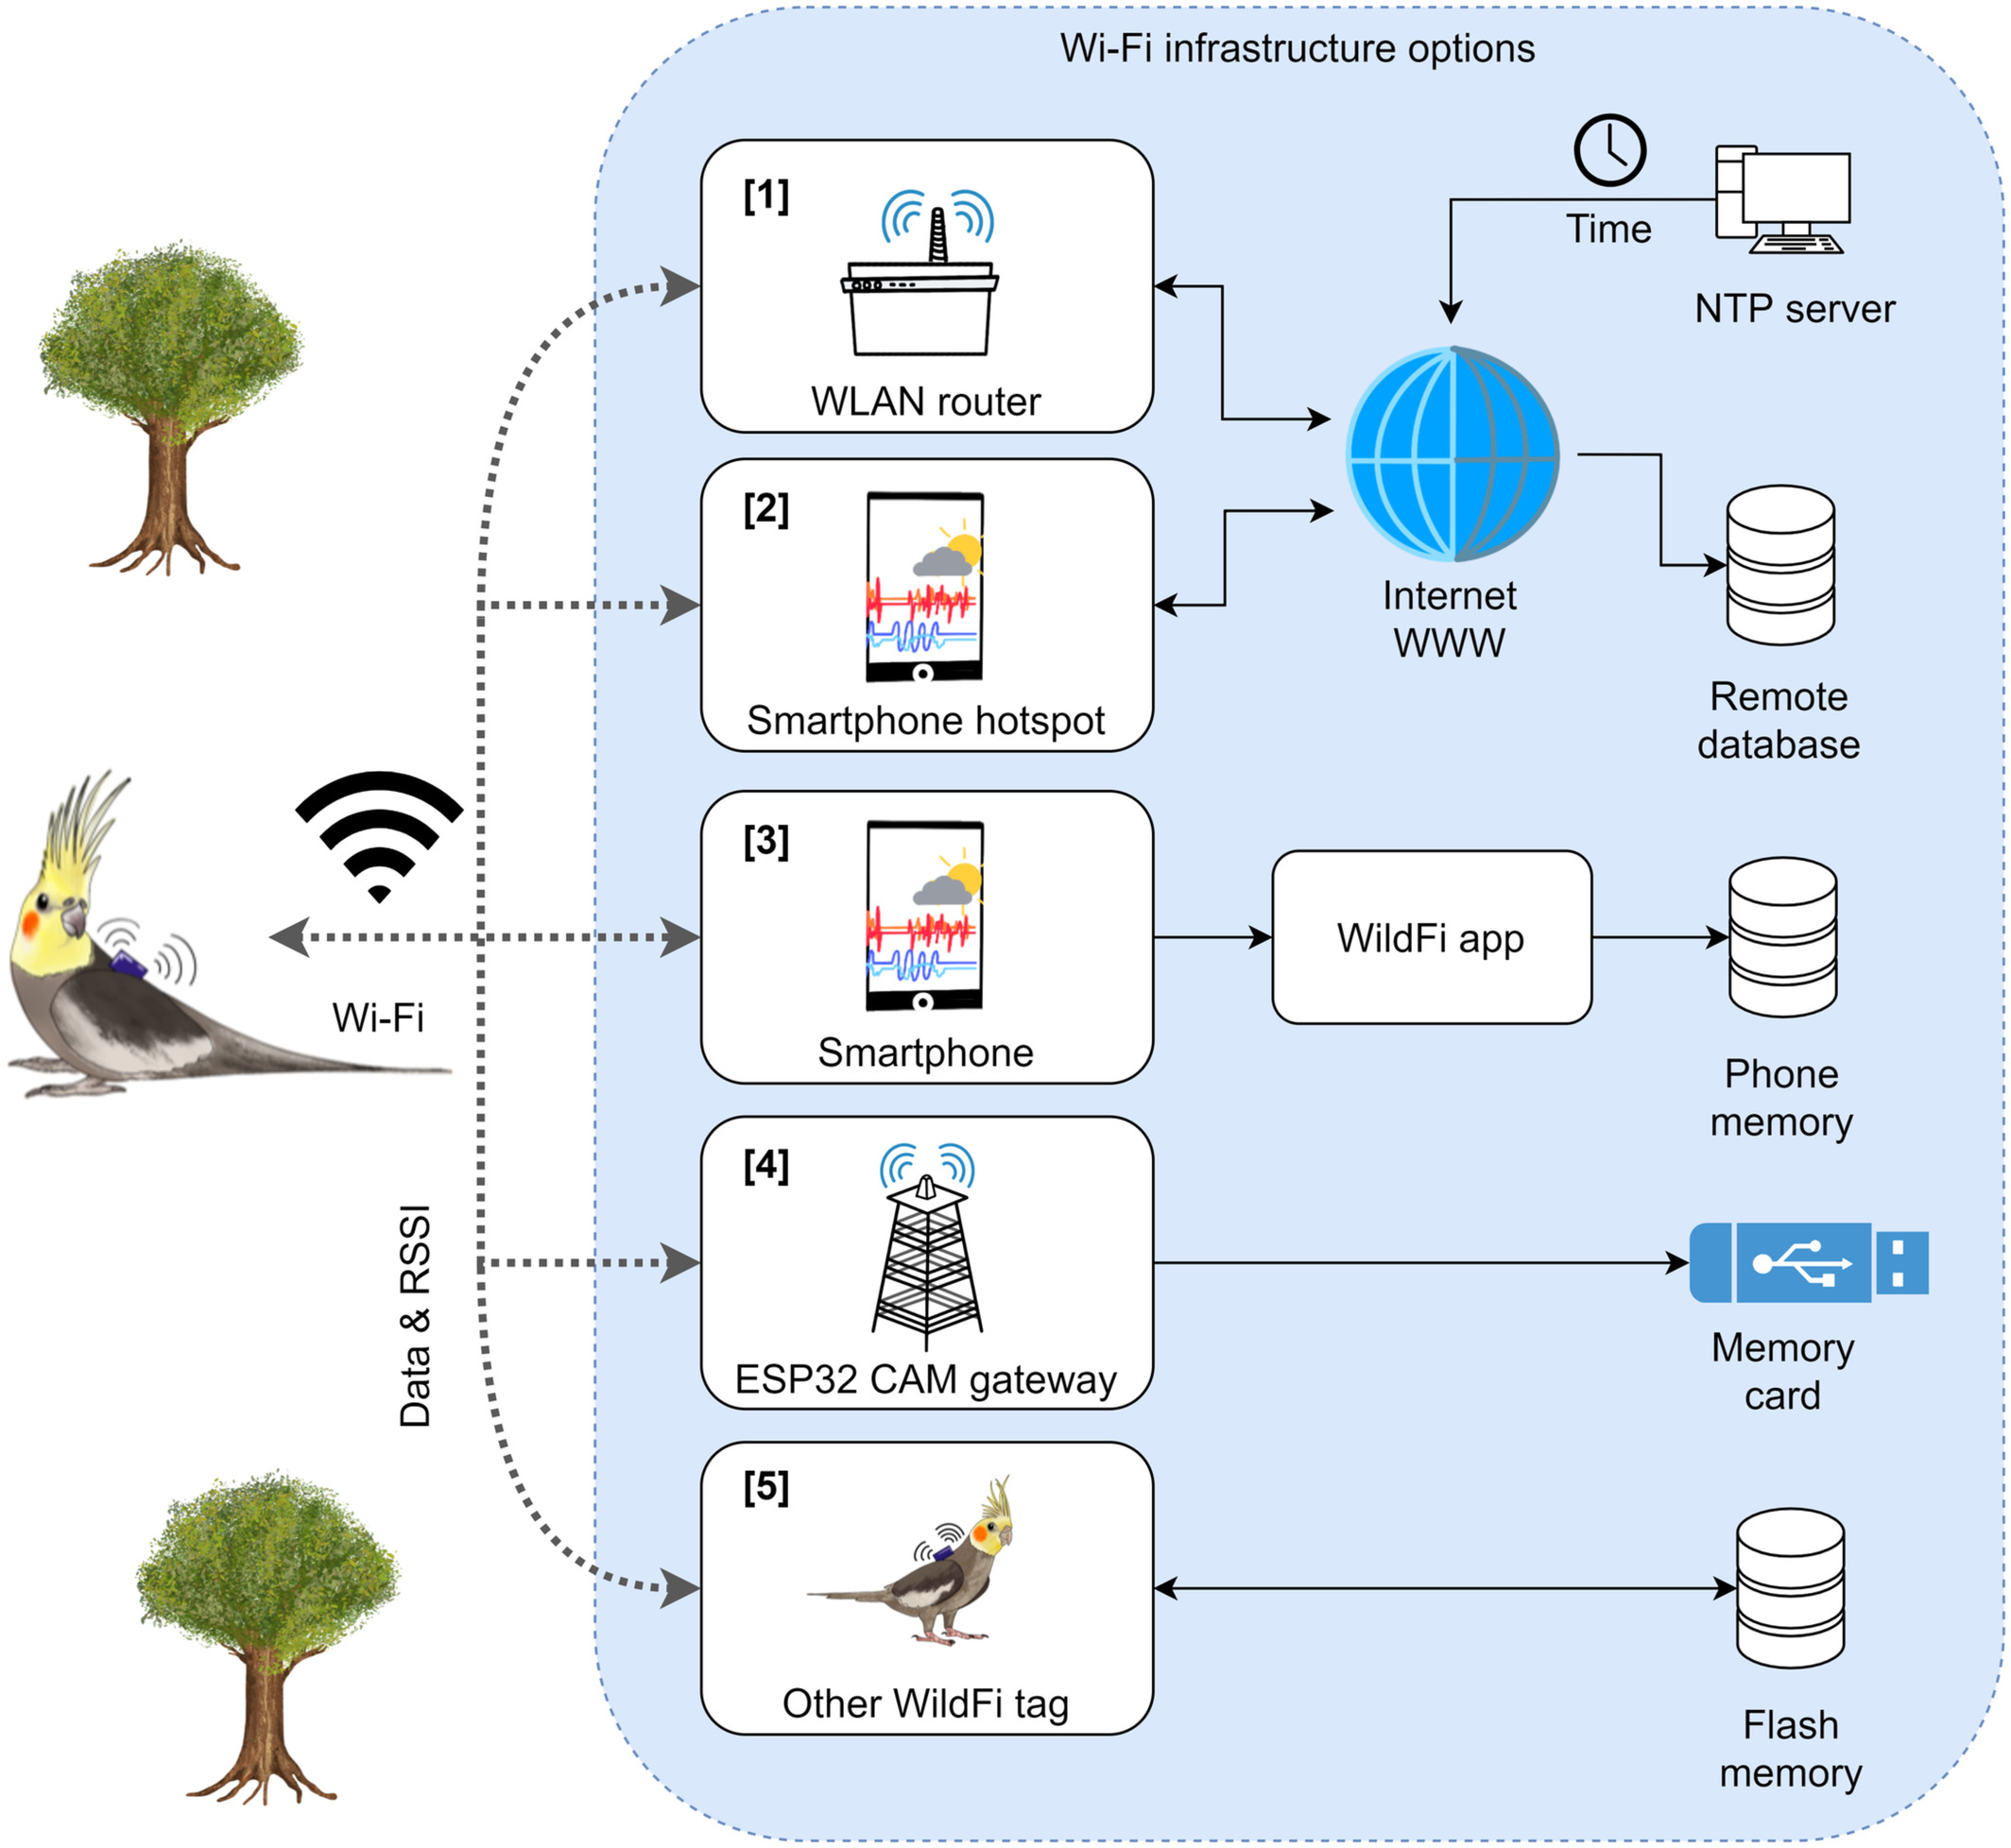
\includegraphics[width=\textwidth]{WildFi_IoT.jpg}
          \caption{WildFi infrastructure overview \cite{wild2023internet}}
          \label{fig:WildFi_infrastructure_overview}
        \end{figure}
      \end{column}
    \end{columns}
  \end{frame}

  \begin{frame}{Networking}
    \frametitle{WLAN Operation}
    \begin{columns}
      \begin{column}{0.5\textwidth}
        \begin{figure}[htbp]
          \centering
          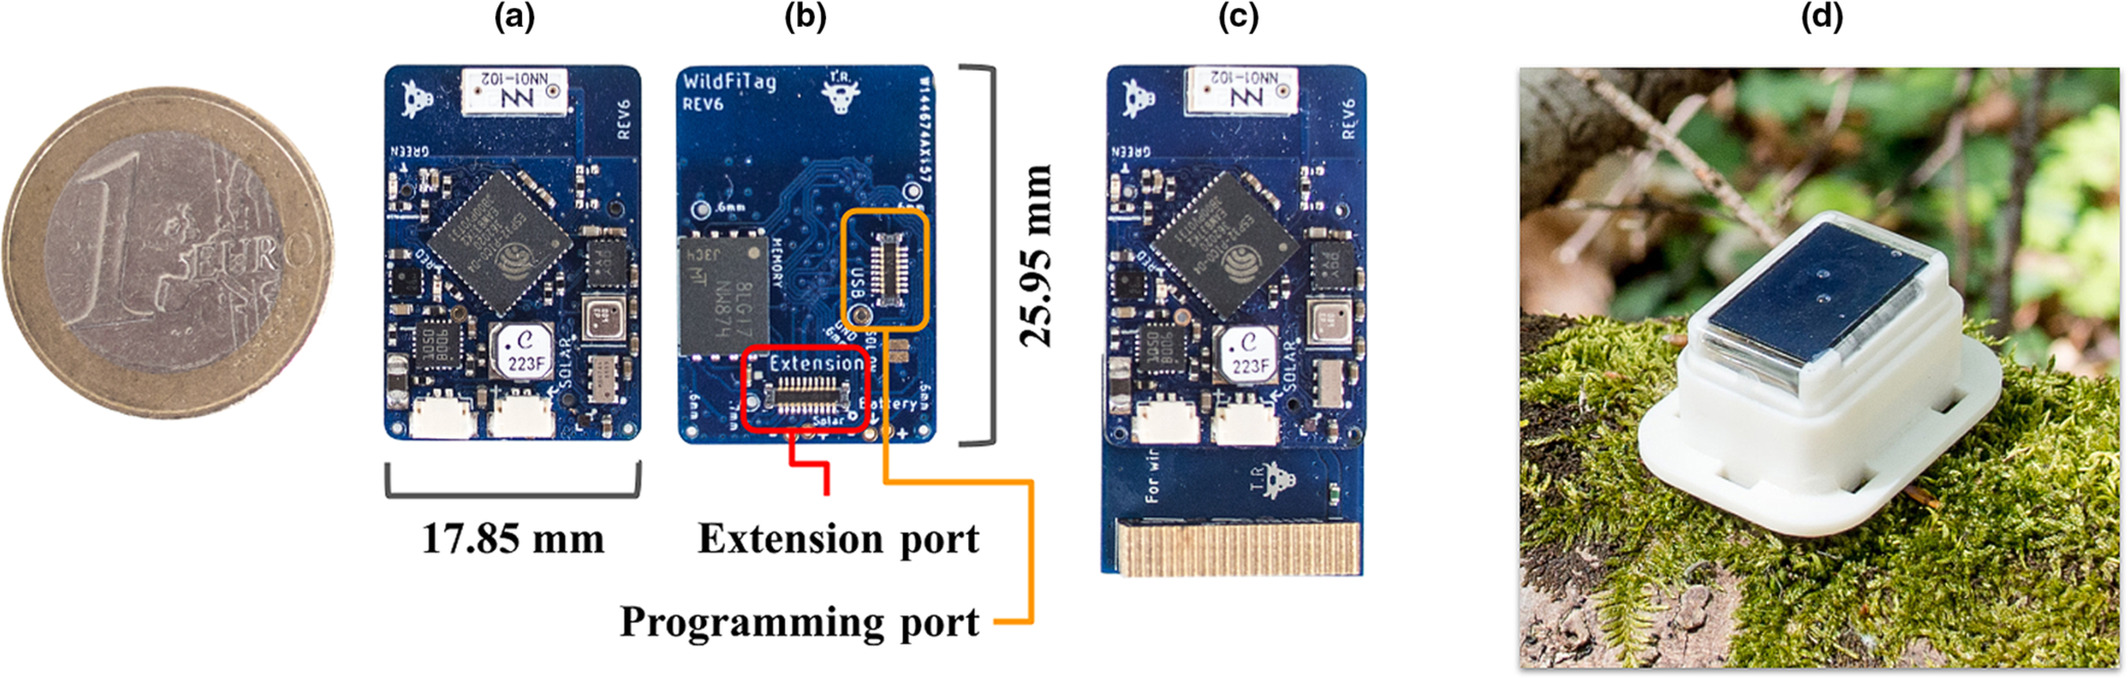
\includegraphics[width=\textwidth]{WildFi_Tag.jpg}
          \caption{WildFi tag with GPS extension and solar panel \cite{wild2023internet}}
          \label{fig:WildFi_Tag}
        \end{figure}
      \end{column}
      \begin{column}{0.5\textwidth}
        \begin{itemize}
          \item Can be entirely self developed
          \item Can last an animals lifetime with solar
          \item Cheap, Open Source, common hardware
          \item Maintained entirely by user
        \end{itemize}
      \end{column}
    \end{columns}
  \end{frame}

\subsection{Security}

  \begin{frame}{Security}
    \frametitle{SigFox and LoRa Security}
    \begin{columns}
      \begin{column}{0.5\textwidth}
        \begin{itemize}
          \item SigFox and LoRa use AES-128
          \item End-to-End encryption
          \item Encrypted at the source (sensor device)
          \item Per device keys for physical protection
        \end{itemize}
      \end{column}
      \begin{column}{0.5\textwidth}
        \begin{figure}[htbp]
          \centering
          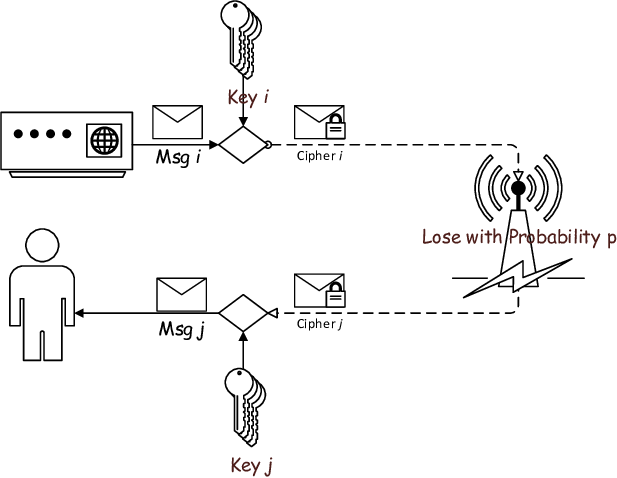
\includegraphics[width=\textwidth]{Model-of-LPWAN-Chaining-Encryption.png}
          \caption{Model of LPWAN Chaining Encryption \cite{bidgoly2019novel}}
          \label{fig:LPWAN_encryption}
        \end{figure}
      \end{column}
    \end{columns}
  \end{frame}

  \begin{frame}{Security}
    \frametitle{WildFi (WLAN) Security}
    \begin{columns}
      \begin{column}{0.5\textwidth}
        \begin{itemize}
          \item WildFi use WPA2/HTTPS $\rightarrow$ AES-128
          \item End-to-End encryption
          \item Depends on individual implementation
        \end{itemize}
      \end{column}
      \begin{column}{0.5\textwidth}
        \begin{figure}[htbp]
          \centering
          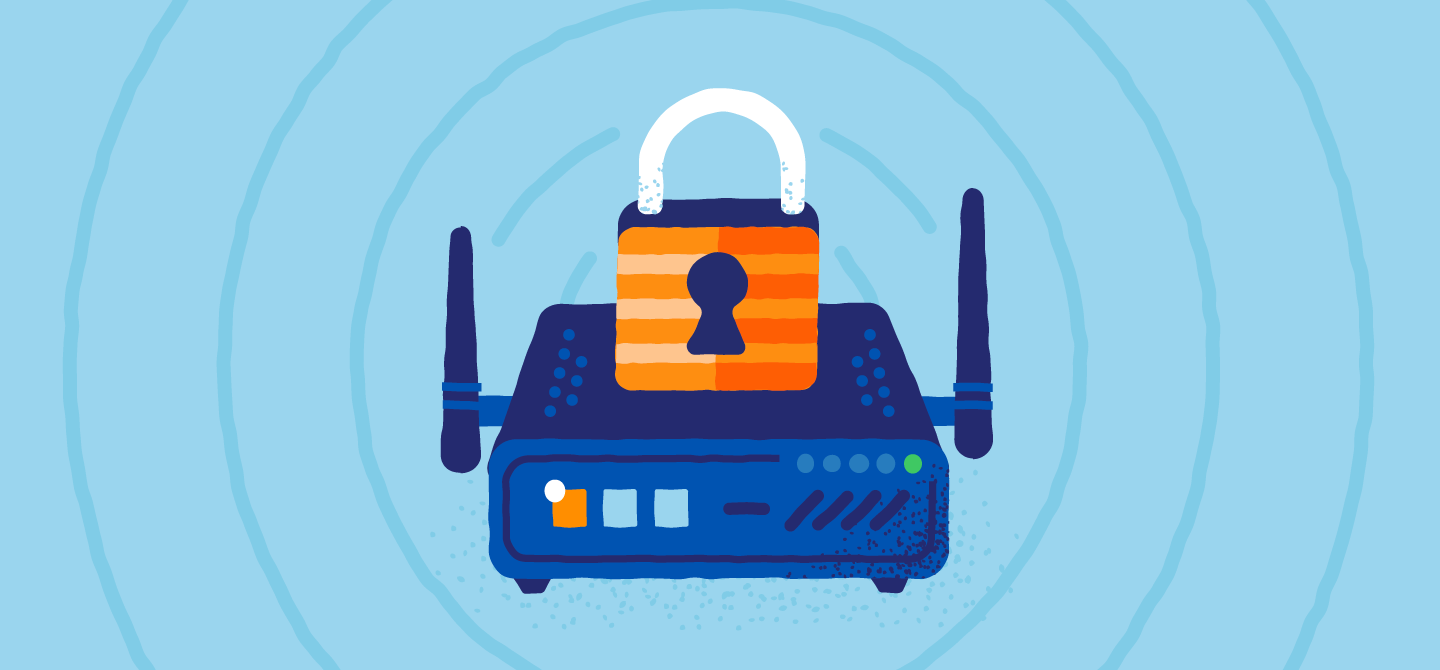
\includegraphics[width=\textwidth]{wireless-router-security.png}
          \label{fig:Wifi_security}
        \end{figure}
      \end{column}
    \end{columns}
  \end{frame}

  \begin{frame}{Security}
    \frametitle{Why Use AES-128?}
    \begin{columns}
      \begin{column}{0.5\textwidth}
        \begin{figure}[htbp]
          \centering
          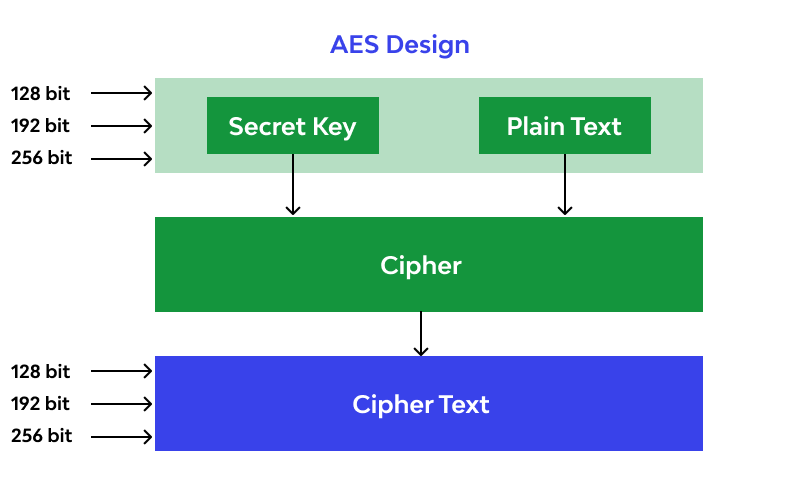
\includegraphics[width=\textwidth]{AES128_structure.png}
          \caption{AES Design \cite{Beschokov}}
          \label{fig:AES_Design}
        \end{figure}
      \end{column}
      \begin{column}{0.5\textwidth}
        \begin{itemize}
          \item Proven track record
          \item Secures data over the air
          \item Small 128bit encryption keys
          \item Not computationally expensive
          \item \faThumbsOUp$ $ Security on battery powered devices
        \end{itemize}
      \end{column}
    \end{columns}
  \end{frame}

\subsection{Comparisons}

\begin{frame}{Comapisons}
  \frametitle{LPWAN Network Comparisons}
  \begin{columns}
    \begin{column}{0.5\textwidth}
      \begin{itemize}
        \item SigFox
        \begin{itemize}
          \item Better range and coverage
          \item Worse latency and payload
        \end{itemize}
        \item LoRa
        \begin{itemize}
          \item Easier to deploy (Private)
          \item Less data restrictions
        \end{itemize}
      \end{itemize}
    \end{column}
    \begin{column}{0.5\textwidth}
      \begin{figure}[htbp]
        \centering
        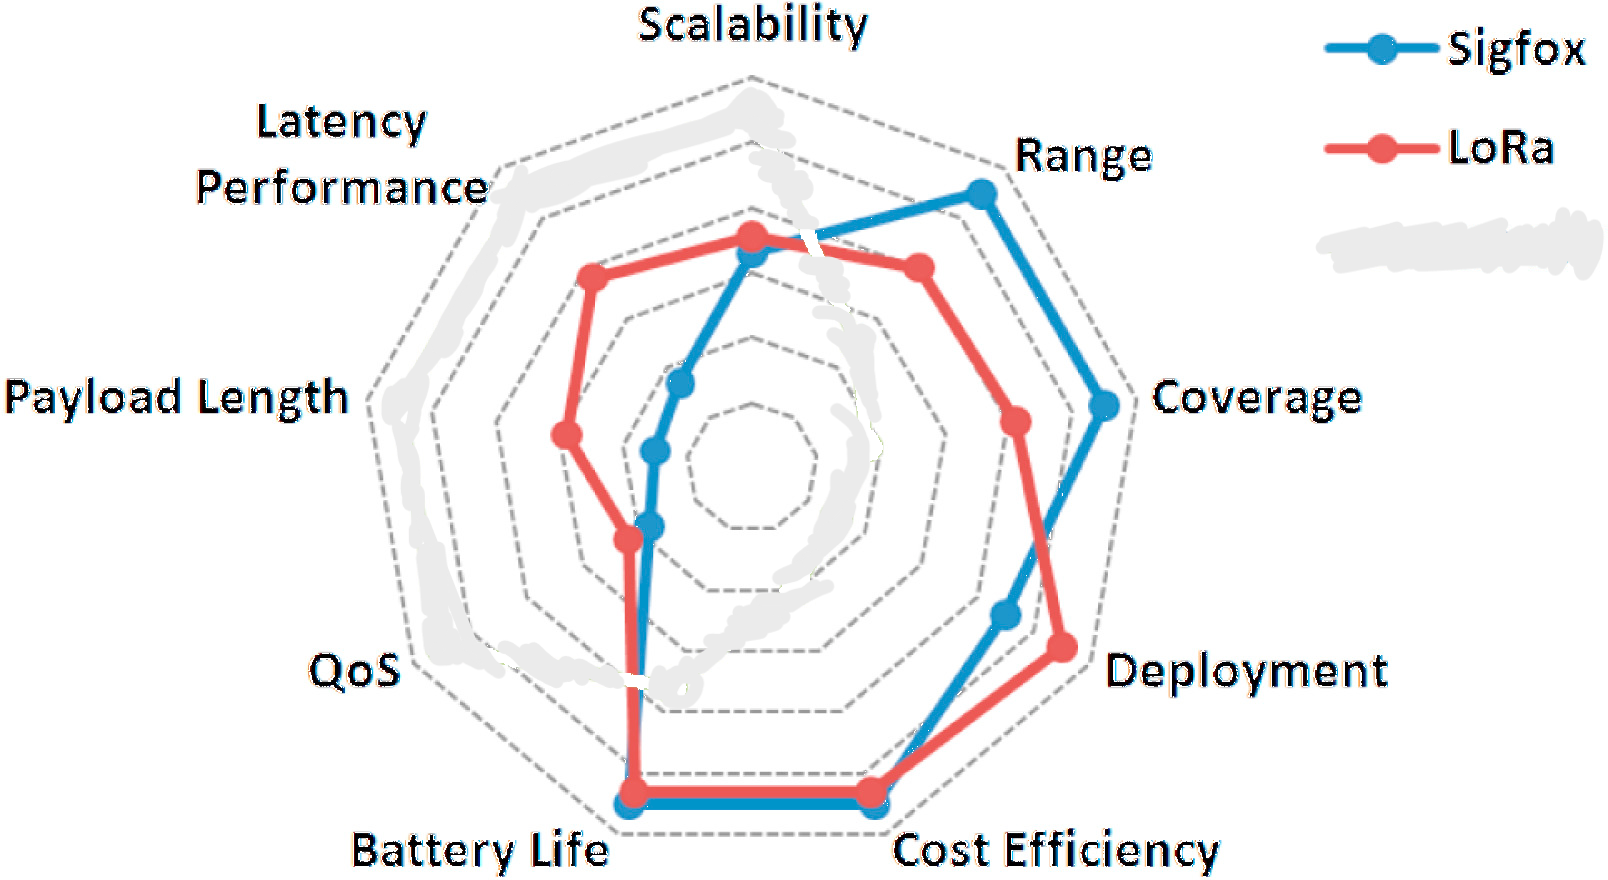
\includegraphics[width=\textwidth]{LPWAN_comparisons.png}
        \caption{LPWAN Comparisons \cite{mekki2019comparative}}
        \label{fig:LPWAN_Comparisons_map}
      \end{figure}
    \end{column}
  \end{columns}
\end{frame}

\begin{frame}{Comparisons}
  \frametitle{LPWAN vs WLAN}
  \begin{columns}
    \begin{column}{0.5\textwidth}
      \begin{figure}[htbp]
        \centering
        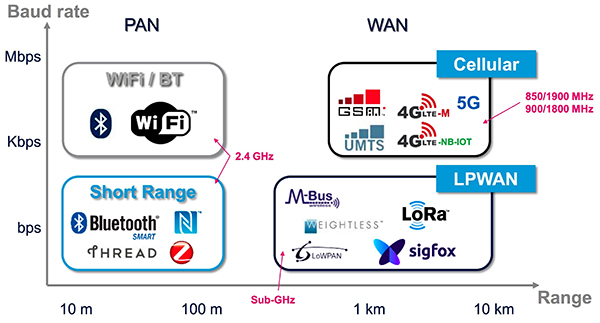
\includegraphics[width=\textwidth]{NetworkRangeDataRateGraph.jpg}
        \caption{Data Rate vs Range \cite{evanczukspeed}}
        \label{fig:Network_range_graph}
      \end{figure}
    \end{column}
    \begin{column}{0.5\textwidth}
      \begin{itemize}
        \item Cost: LoRa \& WLAN $<$ SigFox
        \item Range: LoRa \& SigFox $<$ WLAN
        \item Battery Life: LoRa $\approx$ SigFox $\approx$ WLAN
        \item Data Rate: WLAN $>$ LoRa $>$ SigFox
        \item Security: LoRa $\approx$ SigFox $\approx$ WLAN
      \end{itemize}
    \end{column}
  \end{columns}
\end{frame}

\section{Conclusion}

\begin{frame}{Conclusion}
  \frametitle{IoT for Biologging}
  \begin{columns}
    \begin{column}{0.5\textwidth}
      \begin{itemize}
        \item More, diverse data can be sent
        \item Highly customizable
        \item Many different options to choose from
        \item Lasts for a lifetime
        \item Less disruptive
      \end{itemize}
    \end{column}
    \begin{column}{0.5\textwidth}
      \begin{figure}[htbp]
        \centering
        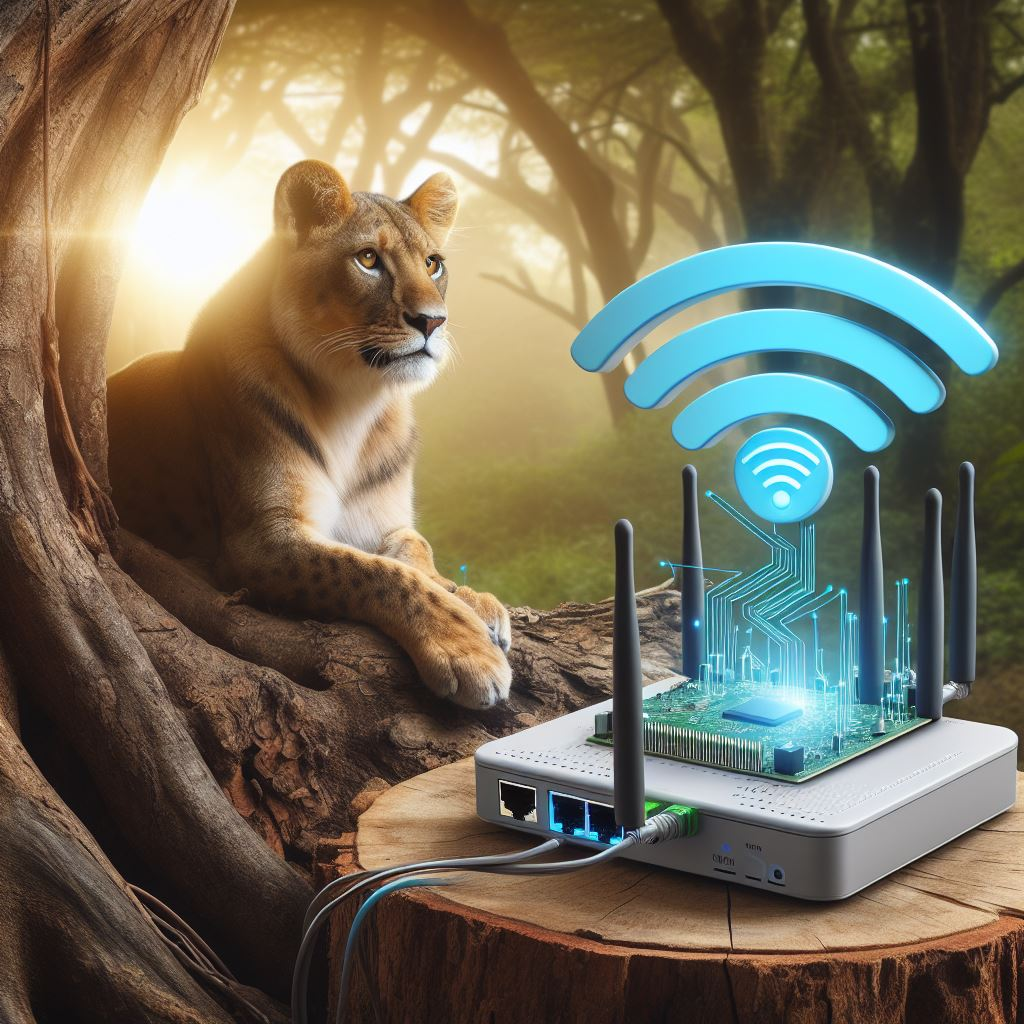
\includegraphics[width=.9\textwidth]{IoT_Lion.jpg}
        \caption{IoT sensor device on an animal in the wild [DALL$\cdot$E 3]}
        \label{fig:IoT_Lion}
      \end{figure}
    \end{column}
  \end{columns}
\end{frame}

\section{Questions}

\begin{frame}{Questions}
  \centering \Large
  \emph{Thanks for Listening!}

  Any Questions?

  \begin{figure}[htbp]
    \centering
    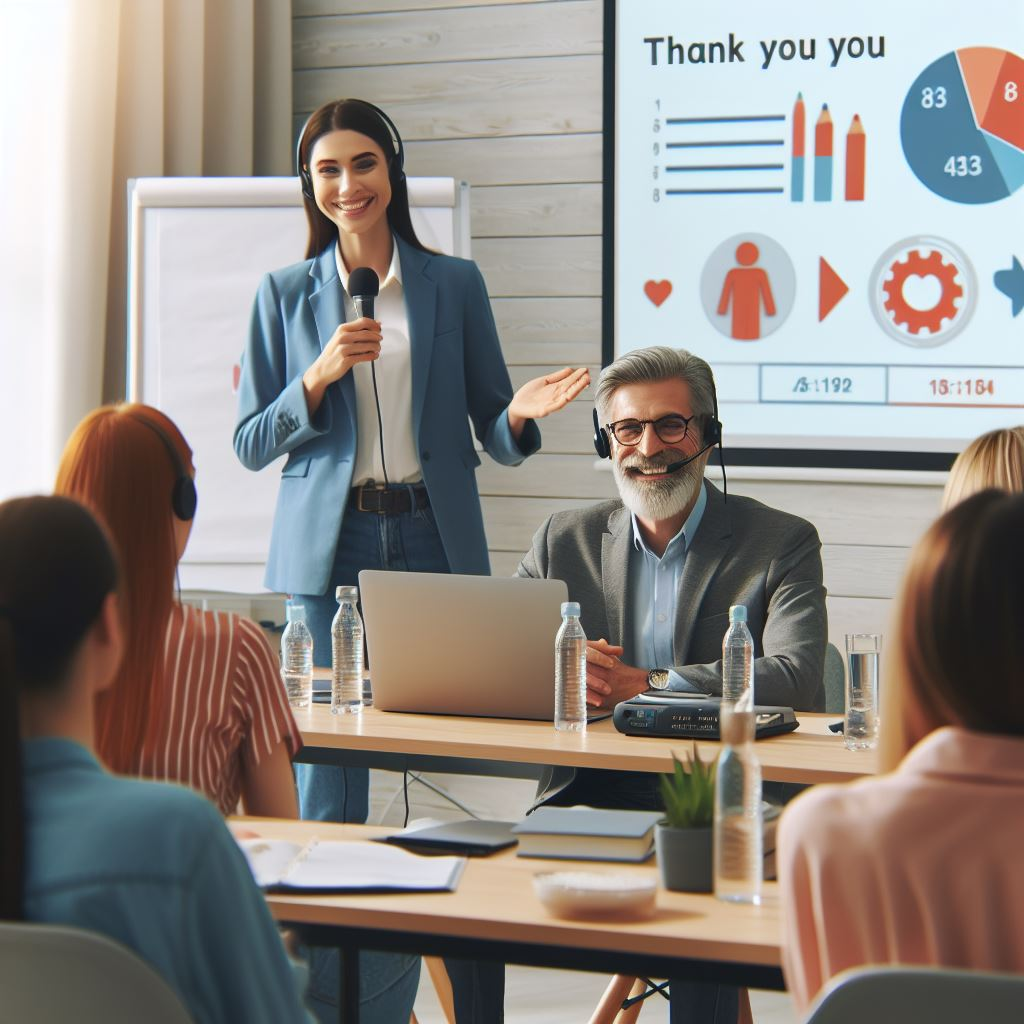
\includegraphics[height=.6\textheight]{Thank_you.jpg}
    \label{fig:Thank_you}
  \end{figure}
\end{frame}

\begin{frame}[allowframebreaks]
  \frametitle{References}
  \printbibliography
\end{frame}


\end{document}